\chapter{Sizing optimization}
After summarizing fundamentals of optimization in previous chapter, we can finally focus on structural optimization problems. In this chapter, we focus on the optimization of discrete truss structures. 

A general procedure to solve such problems involves the following steps:
\begin{enumerate}
    \item Definition of the truss with all nodes, elements, material properties, constraints and initial design choice
    \item Solution of unknown displacements for each node in the truss for the current design
    \item Evaluation of the objective function and its gradients w.r.t. the design variables
    \item Formulation of an MMA approximation and update asymptotes
    \item Solution of the dual problem 
    \item Repetition of steps 1,2,3, and 4 until a maximum of iterations is reached or until there is no improvement of the objective function any more
\end{enumerate}


\begin{objectives}{}{objectives_sizing}
After studying this chapter and finishing the exercise, you should be able to 
\begin{itemize}[label=$\dots$]
    \item explain how general 2D truss problems can be solved employing element stiffness matrices and global stiffness matrices
    \item define an optimization problem to minimize compliance of two-dimensional trusses with volume constraints
    \item explain properties of the aforementioned optimization problem
    \item employ MMA to solve two-dimensional truss optimization problems
\end{itemize}
\end{objectives}

\section{General 2D trusses}
A two-dimensional truss structure is defined by a finite set of $N$ nodes 
\begin{equation}
    \mathcal{N}=\{\mathbf{n}^i \in \mathcal{R}^2, i \in [0, N-1]\}
\end{equation} and a finite set of $M$ element tuples 
\begin{equation}
    \mathcal{E} = \{(\mathbf{n}^0_j, \mathbf{n}^1_j), j \in [0, M-1]\}
\end{equation} 
connecting exactly two nodes $\mathbf{n}^0_j,  \mathbf{n}^1_j \in \mathcal{N}$ each. An example of a two-dimensional truss structure with 10 nodes and 20 elements is shown in Figure \ref{fig:truss_example}.

\begin{figure}[!htpb]
    \centering
    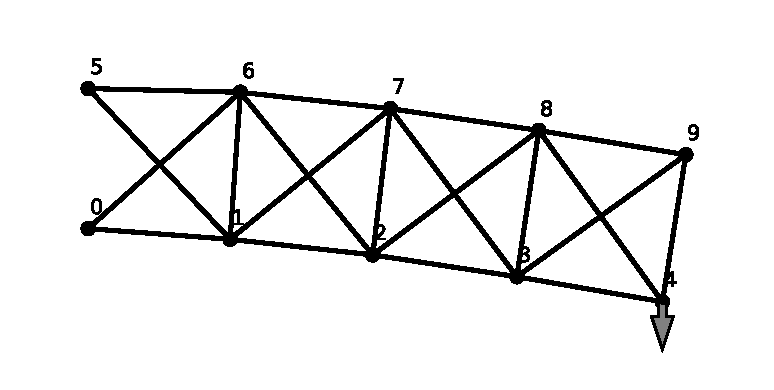
\includegraphics[width=\textwidth]{figures/truss_sample.pdf}
    \caption{Example of a truss with $N=10$ numbered nodes.}
    \label{fig:truss_example}
\end{figure}

In this lecture, all elements transfer only axial forces (positive for tension, negative for compression), have a constant Young's modulus $E$, and have element-wise constant cross sectional areas $a_j$, which will act as design variables later on. Each node has two degrees of freedom to deform $\mathbf{u}^i (\mathbf{a}) \in \mathcal{R}^2$, unless a degree of freedom is constrained by a support. The actual value of each degree of freedom depends on the truss design $\mathbf{a}$. At each node, there may also act an external force $\mathbf{f}^i \in \mathcal{R}^2$, which is independent of the truss design $\mathbf{a}$.

\begin{figure}[!htpb]
    \centering
    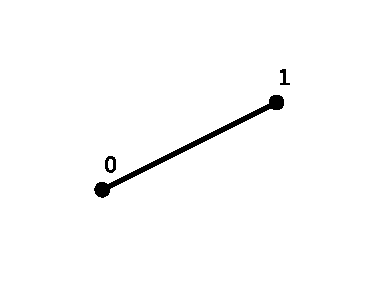
\includegraphics[width=0.4\textwidth]{figures/single_truss.pdf}
    \caption{A single truss element with two nodes.}
    \label{fig:single_truss}
\end{figure}


Without considering optimization for now, we are generally interested in solving the truss problem for the unknown displacements $\mathbf{u}^i(\mathbf{a})$. To do so, we take a look at a single element, like the one shown in Figure \ref{fig:single_truss}. This truss element is defined by two nodes at positions $\mathbf{n}^0_j$ and $\mathbf{n}^1_j$. It has four degrees of freedom 
\begin{equation}
    \mathbf{u}_j (\mathbf{a}) = 
    \begin{pmatrix}
        \mathbf{u}^0_j \\  \mathbf{u}^1_j
    \end{pmatrix}
    = 
    \begin{pmatrix}
        (u_1)^0_j \\ (u_2)^0_j \\  (u_1)^1_j \\ (u_2)^1_j
    \end{pmatrix}
\end{equation} 
and four nodal forces 
\begin{equation}
    \mathbf{f}_j (\mathbf{a}) = 
    \begin{pmatrix}
        \mathbf{f}^0_j \\  \mathbf{f}^1_j
    \end{pmatrix}
    = 
    \begin{pmatrix}
        (f_1)^0_j\\ (f_2)^0_j\\ (f_1)^1_j \\ (f_2)^1_j
    \end{pmatrix},
\end{equation} 
where the notation $\mathbf{u}_j(\mathbf{a}) \in \mathcal{R}^4$ and $\mathbf{f}_j (\mathbf{a}) \in \mathcal{R}^4$ indicates that the solution for displacement degrees of freedom and nodal forces depends on the global design $\mathbf{a}$. 
The displacements can be related to the nodal forces via 
\begin{equation}
    \mathbf{f}_j (\mathbf{a}) = \mathbf{k}_j(a_j) \cdot \mathbf{u}_j (\mathbf{a})
\end{equation}
with an element stiffness matrix $\mathbf{k}_j \in \mathcal{R}^{4\times4}$ defined as 
\begin{equation}
    \mathbf{k}_j(a_j) = a_j \mathbf{k}_j^0 = a_j\frac{E}{l_j}
    \begin{pmatrix}
    \cos{\phi}^2 & \cos{\phi}\sin{\phi} & -\cos{\phi}^2 & -\cos{\phi}\sin{\phi} \\
    \cos{\phi}\sin{\phi} & \sin{\phi}^2 & -\cos{\phi}\sin{\phi} & -\sin{\phi}^2 \\
    -\cos{\phi}^2 & \cos{\phi}\sin{\phi} & \cos{\phi}^2 &\cos{\phi}\sin{\phi} \\
    -\cos{\phi}\sin{\phi} & -\sin{\phi}^2 & \cos{\phi}\sin{\phi} & \sin{\phi}^2 \\
    \end{pmatrix}
\end{equation}
using the orientation angle of the element $\phi = \arctan\left(\frac{n^0_2-n^1_2}{n^0_1-n^1_1}\right)$, the cross sectional area of an element $a_j$, and the length 
\begin{equation}
    l_j = \sqrt{(n^0_2-n^1_2)^2 + (n^0_1-n^1_1)^2}.
\end{equation}
This element stiffness matrix is symmetric and positive semi-definite, i.e. $\mathbf{v} \cdot \mathbf{k}_j(a_j) \cdot \mathbf{v} \ge 0 \hspace{0.5em} \forall \mathbf{v}$. 

Similar, we can denote a relation for all degrees of freedom $\mathbf{u} (\mathbf{a}) \in \mathcal{R}^{2N}$ and all forces $\mathbf{f} \in \mathcal{R}^{2N}$ as 
\begin{equation}
    \mathbf{f} = \mathbf{K}(\mathbf{a}) \cdot  \mathbf{u} (\mathbf{a})
    \label{eq:global_stiffness}
\end{equation}
with a global stiffness matrix $\mathbf{K} (\mathbf{a}) \in \mathcal{R}^{2N \times 2N}$. This global stiffness matrix is assembled from element stiffness matrices by adding entries of all element stiffness matrices at the correct positions. This can be written as 
\begin{equation}
    \underbrace{
    \begin{pmatrix}
        \dots \\ (f_1)^0_j \\ (f_2)^0_j \\ \dots \\ (f_1)^1_j \\ (f_2)^1_j \\ \dots \\
    \end{pmatrix}}_{\mathbf{f}}
    =
    \underbrace{
    \sum_j
    \underbrace{
    \begin{pmatrix}
    \dots & \dots & \dots & \dots & \dots & \dots & \dots \\
    \dots & (k_{11})_j & (k_{12})_j & \dots & (k_{13})_j & (k_{14})_j & \dots  \\
    \dots & (k_{21})_j & (k_{22})_j & \dots & (k_{23})_j & (k_{24})_j & \dots  \\
    \dots & \dots & \dots & \dots & \dots & \dots & \dots  \\
    \dots & (k_{31})_j & (k_{32})_j & \dots & (k_{33})_j & (k_{34})_j & \dots  \\
    \dots & (k_{41})_j & (k_{42})_j & \dots & (k_{43})_j & (k_{44})_j & \dots  \\
    \dots & \dots & \dots & \dots & \dots & \dots & \dots  \\
    \end{pmatrix}}_{\mathbf{K}_j (a_j) = a_j \mathbf{K}^0_j }
    }_{\mathbf{K}(\mathbf{a})}
    \underbrace{
    \begin{pmatrix}
        \dots \\ (u_1)^0_j \\ (u_2)^0_j \\ \dots \\ (u_1)^1_j \\ (u_2)^1_j \\ \dots \\
    \end{pmatrix}}_{\mathbf{u} (\mathbf{a})},
\end{equation}
where the degrees of freedom $(u_1)^0_j, (u_2)^0_j$ etc. are at the positions in the vector corresponding to the global node displacements $\mathbf{u} (\mathbf{a})$. The matrices $\mathbf{K}_j(a_j)$ are zero everywhere except for the 16 positions at which they are filled with values from $\mathbf{k}_j(a_j)$. They are linear in $a_j$, hence we can write $\mathbf{K}_j(a_j) = a_j \mathbf{K}^0_j$, where $\mathbf{K}^0_j$ does not depend on $a_j$.
The global stiffness matrix is symmetric and positive semi-definite, just like the element stiffness matrix.

Before solving the global system of equations, we need to remove those entries containing constrained degrees of freedom. This is achieved by simply removing all constrained entries in $\mathbf{f}$ and $\mathbf{u}(\mathbf{a})$ and the corresponding rows and columns in the global stiffness matrix $\mathbf{K}(\mathbf{a})$. If we do not remove sufficient degrees of freedom, the matrix would be singular and cannot be solved. The physical interpretation of this behavior is simple: The truss is statically undetermined and can move freely. 

Finally, we end up with a reduced system of equations 
\begin{equation}
     \mathbf{f}_\textrm{red} = \mathbf{K}_\textrm{red}(\mathbf{a})  \cdot \mathbf{u}_\textrm{red} (\mathbf{a})
     \label{eq:reduced_system}
\end{equation}
where $\mathbf{K}_\textrm{red}(\mathbf{a})$ is strictly positive definite and not singular (if sufficient boundary conditions have been applied). Solving this system of equation gives us the unknown node displacements. 

As a post-processing step, we may compute the strain energy per area in each element 
\begin{equation}
    w_j = \frac{1}{2}\mathbf{u}_j (\mathbf{a}) \cdot \mathbf{k}^0_j \cdot \mathbf{u}_j (\mathbf{a}) = \frac{1}{2} \frac{S_j^2}{E} l_j
    \label{eq:element_strain_energy}
\end{equation}
or the stress in each element 
\begin{equation}
    S_j = \frac{E}{l_j} 
    \begin{pmatrix}
        \cos{\phi} & \sin{\phi} & -\cos{\phi} & \sin{\phi}
    \end{pmatrix}
    \cdot 
    \mathbf{u}_j(\mathbf{a}).
\end{equation}

An exemplary solution for the example shown in Figure \ref{fig:truss_example} is given in Figure \ref{fig:truss_example_solved} with colors indicating the stresses in trusses. For this computation, it was assumed that all cross sections are identical.

\begin{figure}[!htpb]
    \centering
    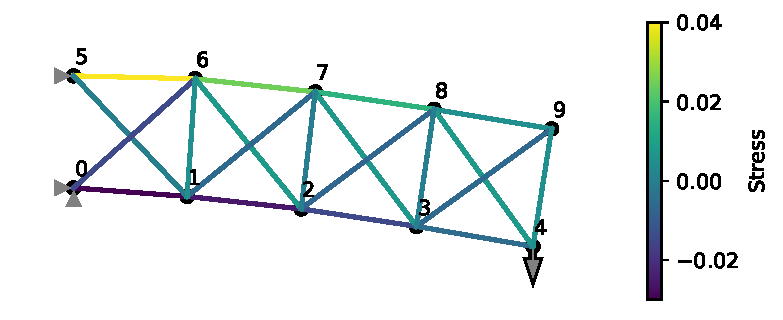
\includegraphics[width=\textwidth]{figures/truss_sample_solved.pdf}
    \caption{Exemplary solution of a truss computation for the example shown in Figure \ref{fig:truss_example}.}
    \label{fig:truss_example_solved}
\end{figure}

\begin{example}{Three bar truss}{trussexample}
    Consider the truss shown below, which is subjected to a force $P$ indicated by the gray arrow and supports indicated by gray triangles. It has three nodes 
    \begin{equation}
        \mathcal{N} = \{\mathbf{n}^0=(1,0)^\top, \mathbf{n}^1=(0,0)^\top,\mathbf{n}^2=(0,1)^\top \}
    \end{equation}
    and three elements 
    \begin{equation}
        \mathcal{E} = \{(\mathbf{n}^0, \mathbf{n}^1), (\mathbf{n}^0, \mathbf{n}^2), (\mathbf{n}^1, \mathbf{n}^2)\}.
    \end{equation}

    \begin{center}
        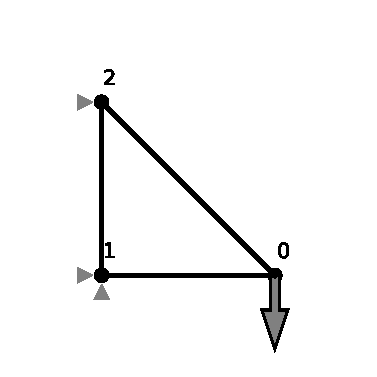
\includegraphics[width=0.5\textwidth]{figures/three_bar_truss.pdf}
    \end{center}

    The element stiffness matrices are 
    \begin{equation}
        \mathbf{K}_0(a_0) = E a_0
        \begin{pmatrix}
             1 & 0 & -1 & 0 \\
             0 & 0 &  0 & 0 \\
            -1 & 0 &  1 & 0 \\
             0 & 0 &  0 & 0
        \end{pmatrix},
    \end{equation}
    \begin{equation}
        \mathbf{K}_1(a_1) = \frac{E a_1}{2\sqrt{2}}
        \begin{pmatrix}
             1 & -1 & -1 &  1 \\
            -1 &  1 &  1 & -1 \\
            -1 &  1 &  1 & -1 \\
             1 & -1 & -1 &  1
        \end{pmatrix}
    \end{equation}
    and 
    \begin{equation}
        \mathbf{K}_2(a_2) = E a_2
        \begin{pmatrix}
            0 &  0 & 0 &  0 \\
            0 &  1 & 0 & -1 \\
            0 &  0 & 0 &  0 \\
            0 & -1 & 0 &  1 
        \end{pmatrix}.
    \end{equation}

    The global stiffness matrix is 
    \begin{equation}
        \mathbf{K}(a) = E
        \begin{pmatrix}
             a_0 + \frac{a_1}{2\sqrt{2}}&  -\frac{a_1}{2\sqrt{2}} & \cellcolor{aux_green!10}-a_0 &  \cellcolor{aux_green!10}0 & -\cellcolor{aux_green!10} \frac{a_1}{2\sqrt{2}} &  \frac{a_1}{2\sqrt{2}}\\
            -\frac{a_1}{2\sqrt{2}} &  \frac{a_1}{2\sqrt{2}} & \cellcolor{aux_green!10} 0 & \cellcolor{aux_green!10} 0 & \cellcolor{aux_green!10}\frac{a_1}{2\sqrt{2}} &  -\frac{a_1}{2\sqrt{2}} \\
            \rowcolor{aux_green!10}
             -a_0 &  a_0 & 0 &  0 & 0 & 0\\
             \rowcolor{aux_green!10}
            0 &  0 & 0 &  a_2 & 0 &  -a_2 \\
            \rowcolor{aux_green!10}
             -\frac{a_1}{2\sqrt{2}} &  \frac{a_1}{2\sqrt{2}} & 0 &  0 & \frac{a_1}{2\sqrt{2}} &  -\frac{a_1}{2\sqrt{2}}\\
            \frac{a_1}{2\sqrt{2}} &  -\frac{a_1}{2\sqrt{2}} & \cellcolor{aux_green!10} 0 &  \cellcolor{aux_green!10} -a_2 & \cellcolor{aux_green!10} -\frac{a_1}{2\sqrt{2}} &  a_2 + \frac{a_1}{2\sqrt{2}}\\
        \end{pmatrix}
    \end{equation}
    with colored rows and columns indicating those entries which will be removed due to constraints. This leads to the reduced system 
    \begin{equation}
        \begin{pmatrix}
            0 \\ -P \\ 0  \\
        \end{pmatrix}
         = E
        \begin{pmatrix}
             a_0 + \frac{a_1}{2\sqrt{2}}&  -\frac{a_1}{2\sqrt{2}} &  \frac{a_1}{2\sqrt{2}}\\
            -\frac{a_1}{2\sqrt{2}} &  \frac{a_1}{2\sqrt{2}} &  -\frac{a_1}{2\sqrt{2}} \\
            \frac{a_1}{2\sqrt{2}} &  -\frac{a_1}{2\sqrt{2}} &  a_2 + \frac{a_1}{2\sqrt{2}}
        \end{pmatrix}
        \mathbf{u}_\textrm{red} (\mathbf{a})
    \end{equation}
    which can be solved for 
    \begin{equation}
        \mathbf{u}_\textrm{red} (\mathbf{a}) = 
        \begin{pmatrix}
            -\frac{P}{Ea_0} \\  \frac{2\sqrt{2}P}{Ea_2} - \frac{P}{Ea_0} - \frac{P}{Ea_1} \\ -\frac{P}{Ea_1}  \\
        \end{pmatrix}
    \end{equation}

    The final result of the computation is shown below.
    
    \begin{center}
        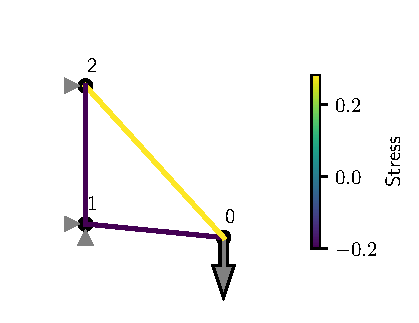
\includegraphics[width=0.5\textwidth]{figures/three_bar_truss_solved.pdf}
    \end{center}    
\end{example}


\section{The standard structural optimization problem}
One possible objective in truss optimization is the search for the cross sectional areas $\mathbf{a}$ resulting in the stiffest truss. The corresponding objective function could be simply the displacement at a specific node or a global displacement measure $\mathbf{u} (\mathbf{a}) \cdot \mathbf{u} (\mathbf{a})$. However, we choose to minimize the compliance $C: \mathcal{R}^{2N} \rightarrow \mathcal{R}$ defined as 
\begin{equation}
    C(\mathbf{a}) = \mathbf{f} \cdot \mathbf{u}(\mathbf{a})
\end{equation} 
of the truss instead. The minimal compliance results also in the stiffest truss, but this formulation is preferred over the pure displacement formulation, because $C(\mathbf{a})$ is convex \cite{Svanberg1984}. The convexity is proven by showing that the Hessian $\nabla^2 C(\mathbf{a})$ is positive semi-definite, a property that is inherited from the positive semi-definiteness of $\mathbf{K}(\mathbf{a})$ (see Chapter 5.2.1 in \cite{Christensen2008} for details).

We employ box constraints $\mathcal{A}$ on the upper and lower limit of the design variables. The upper limit $\mathbf{a}^u$ could be a manufacturing constraint that prevents very thick elements. The lower limit $\mathbf{a}^l$ should be larger than $0$ to prevent deletion of truss elements. If the cross sectional area of all elements connected to a node would become $0$, i.e. all trusses are deleted, the displacement of that node would be undetermined and the stiffness matrix would become singular. In this chapter, we prevent this by demanding $a_j^l > \epsilon > 0$.

A typical inequality constraint is a volume constraint for the total truss volume used in the assembly. If we would not have a volume constraint, the optimization would predict a trivial solution with all cross sections at their maximum area. However, we are interested in solutions that put a limited material resource to its best use and thus limit the total volume to be 
\begin{equation}
    \mathbf{a} \cdot \mathbf{l} \le V_0
\end{equation}
where $V_0$ describes the maximum volume used in the design
In order to find a solution at all, we must obviously choose $V_0 \ge \mathbf{a}^l \cdot \mathbf{l}$, otherwise it would be impossible to find any $\mathbf{a}$ fulfilling the constraint. 

In conclusion, the standard truss optimization problem may be noted as follows:

\begin{equation}
    \begin{aligned}
        \min_{\mathbf{a}} \quad & C(\mathbf{a}) = \mathbf{f} \cdot \mathbf{u}(\mathbf{a})\\
        \textrm{s.t.} \quad & \mathbf{a} \cdot \mathbf{l} - V_0 \le 0  \\
                            & \mathbf{a} \in \mathcal{A}\\
    \end{aligned}
    \label{eq:size_optimization}
\end{equation}

\section{Analysis of the standard optimization problem}
The objective function $C(\mathbf{a})$ is convex, the inequality constraint $\mathbf{a} \cdot \mathbf{l} - V_0$ is convex, and the set $\mathcal{A}$ is compact and convex. Therefore, finding a KKT point is equivalent to finding the global unique solution of the problem. We can denote the Lagrangian 
\begin{equation}
    \mathcal{L}(\mathbf{a}, \mu) = C(\mathbf{a}) + \mu \left( \mathbf{a} \cdot \mathbf{l} - V_0 \right) 
\end{equation}
and need to compute the gradient $\frac{\partial \mathcal{L}}{\partial a_j}$ to solve the optimization problem with Lagrangian duality. This gradient is 
\begin{equation}
    \frac{\partial \mathcal{L} (\mathbf{a}, \mu)}{\partial a_j} 
    = \frac{\partial C (\mathbf{a})}{\partial a_j} + \mu l_j
    = \mathbf{f} \cdot \frac{\partial \mathbf{u} (\mathbf{a})}{\partial a_j} + \mu l_j,
    \label{eq:lagrange_truss_problem}
\end{equation}
where the gradient $\frac{\partial \mathbf{u} (\mathbf{a})}{\partial a_j}$ remains to be determined. It can be obtained by differentiating Equation \eqref{eq:global_stiffness} as
\begin{align}
        && \frac{\partial}{\partial a_j} \mathbf{f} &= \frac{\partial}{\partial a_j} \left( \mathbf{K} (\mathbf{a}) \cdot \mathbf{u} (\mathbf{a}) \right) \\
        \Leftrightarrow &&
        0 &= \frac{\partial \mathbf{K} (\mathbf{a})}{\partial a_j} \cdot \mathbf{u} (\mathbf{a}) + \mathbf{K} (\mathbf{a}) \cdot \frac{\partial \mathbf{u} (\mathbf{a})}{\partial a_j} \\
        \Leftrightarrow &&
        \frac{\partial \mathbf{u} (\mathbf{a})}{\partial a_j} &= - \mathbf{K}^{-1}(\mathbf{a}) \cdot \frac{\partial \mathbf{K} (\mathbf{a})}{\partial a_j}  \cdot \mathbf{u} (\mathbf{a}) \\
        \Leftrightarrow &&
        \frac{\partial \mathbf{u} (\mathbf{a})}{\partial a_j} &= - \mathbf{K}^{-1}(\mathbf{a}) \cdot \frac{\partial \sum_k a_k\mathbf{K}^0_k}{\partial a_j}  \cdot \mathbf{u} (\mathbf{a}) \\
        \Leftrightarrow &&
        \frac{\partial \mathbf{u} (\mathbf{a})}{\partial a_j} &= - \mathbf{K}^{-1}(\mathbf{a}) \cdot \mathbf{K}^0_j \cdot \mathbf{u} (\mathbf{a}).
\end{align}
Substituting this expression into the previous Equation \eqref{eq:lagrange_truss_problem} gives us the sensitivity of the compliance with respect to the design variables 
\begin{align}
    \frac{\partial C (\mathbf{a})}{\partial a_j} 
    &= - \mathbf{f} \cdot \mathbf{K}^{-1}(\mathbf{a}) \cdot \mathbf{K}^0_j \cdot \mathbf{u} (\mathbf{a})  \\
    &= - \mathbf{u} (\mathbf{a}) \cdot \mathbf{K}^0_j \cdot \mathbf{u} (\mathbf{a})  \\
    &= - \mathbf{u}_j (\mathbf{a}) \cdot \mathbf{k}^0_j \cdot \mathbf{u}_j (\mathbf{a})  \\
    &= - 2 w_j (\mathbf{a})
    \label{eq:compliance_sensitivity}
\end{align}
with the strain energy per area in each element $w_j \ge 0$. The strain energy is always greater or equal to zero due to the positive semi-definiteness of $\mathbf{k}^0_j$.
What we have just done is called a \emph{sensitivity analysis} - we obtained an expression of how much a change of variable $a_j$ contributes to the change of the Lagrangian $\frac{\partial \mathcal{L} (\mathbf{a}, \mu)}{\partial a_j}$. It is very valuable to have an analytical expression of the sensitivity, as solving it numerically via finite differences causes a high computational cost and loss in precision.
Finally, the gradient of the Lagrangian becomes 
\begin{equation}
    \frac{\partial \mathcal{L} (\mathbf{a}, \mu)}{\partial a_j} 
    = - 2 w_j (\mathbf{a}) + \mu l_j
    \label{eq:lagrange_sensitivity}
\end{equation}

If we could solve this expression for $\mathbf{a}^*(\mu)$ at the stationary point of the Lagrangian, we could use Lagrangian duality to compute the solution easily. Unfortunately, the solution is not easy, as $w_j$ depends on the global design $\mathbf{a}$ and not just on the design variable in its element $a_j$. For this reason, we will use MMA to solve the problem in the next section.

However, we can still learn something about the solution if we consider Equation \eqref{eq:element_strain_energy}. If we substitute it in Equation \eqref{eq:lagrange_sensitivity}, we can write 
\begin{equation}
    \frac{\partial \mathcal{L} (\mathbf{a}, \mu)}{\partial a_j} = - \frac{S^2_j}{E} l_j + \mu l_j
\end{equation}
and conclude that for an optimal point $\mathbf{a}^l < \mathbf{a}^* < \mathbf{a}^u$ with $\mu^*>0$, i.e. the maximum volume $V_0$ is used and box constraints are not reached, all stress magnitudes are identical with
\begin{equation}
    S_j = \pm \sqrt{\frac{\mu^*}{E}}.
\end{equation}

This is called a \emph{fully stressed design} and is related to a theorem by Australian engineer A.G.M. Michell published in 1904 \cite{Michell1904}. The theorem states that elements of an optimal truss structure lie along the principal directions of a virtual stress field, such that all of them experience an equal stress magnitude \cite{Arora2019}.
An example for a Michell truss structure is given in Figure \ref{fig:michell}.

\begin{figure}[!htpb]
    \centering
    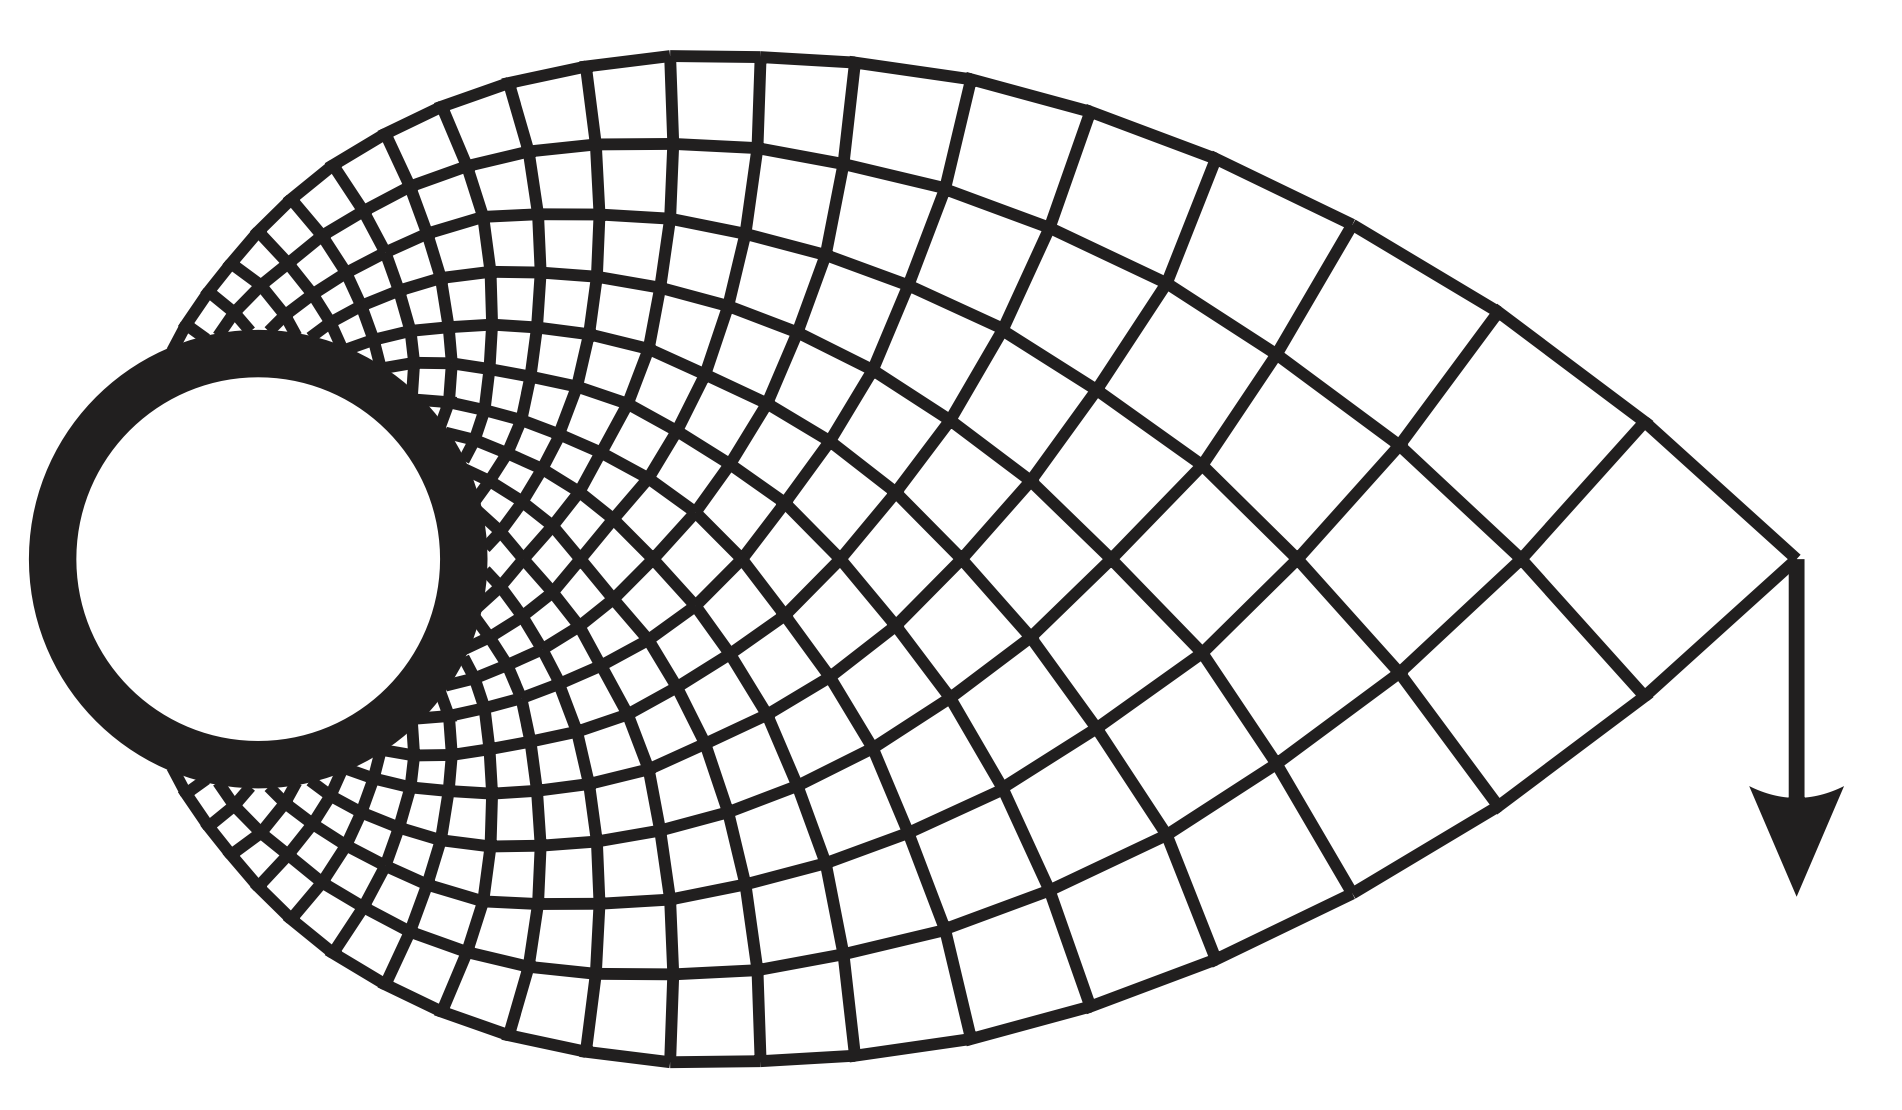
\includegraphics[width=0.5\textwidth]{figures/michell.png}
    \caption{Example of a Michell truss \cite{Picelli2015}. All truss elements in this design experience the same stress magnitude (either in compression or in tension).}
    \label{fig:michell}
\end{figure}

\section{Approximation of the standard optimization problem with MMA}
\label{sec:sizing:mma}

The standard optimization problem for trusses is convex, but it is not separable and explicit, because we cannot find an explicit expression for $\mathbf{a}^*(\mu)$ at the stationary point of the Lagrangian. Therefore we linearize the problem using MMA in $1/(a_j-L_j^k)$. The linearization of the objective function becomes
\begin{align}
    \tilde{C}(\mathbf{a}) &= C(\mathbf{a}^k) + \sum_j \frac{\partial C}{\partial a_j}(\mathbf{a}^k) (a^k_j-L^k_j) - \sum_j \frac{\partial C}{\partial a_j}(\mathbf{a}^k) \frac{(a^k_j-L^k_j)^2}{a_j-L^k_j}\\
    &=C(\mathbf{a}^k) 
    - \sum_j 2w_j (\mathbf{a}^k) (a^k_j-L^k_j)
    + \sum_j 2w_j (\mathbf{a}^k)
    \frac{(a^k_j-L^k_j)^2}{a_j-L^k_j}.
\end{align}
Note that this is a linearization using lower asymptotes only, because 
\begin{equation}
    \frac{\partial C }{\partial a_j}(\mathbf{a}^k)  = - 2 w_j (\mathbf{a}^k) < 0 \quad \forall \mathbf{a}^k
\end{equation} 
and thus all terms in Equations \eqref{eq:mma_start} and \eqref{eq:mma_end} involving $p_j^k$ vanish.
The approximated optimization problem becomes 
\begin{equation}
    \begin{aligned}
        \min_{\mathbf{a}} \quad & \tilde{C} (\mathbf{a})\\
        \textrm{s.t.} \quad & \mathbf{a} \cdot \mathbf{l} - V_0 \le 0  \\
                            & \tilde{\mathbf{a}}^k_l \le \mathbf{a} \le \mathbf{a}^u\\
    \end{aligned}
\end{equation}
with lower move limits $\tilde{\mathbf{a}}^{l,k} = \max(\mathbf{a}^l,  0.9 \mathbf{L}^k + 0.1 \mathbf{a}^k)$ preventing division by zero. The constraint is already linear and thus we do not approximate it.

\section{Solution of the approximated standard optimization problem}
\label{sec:sizing:solution}
The Lagrangian of the approximated problem with Lagrangian duality
\begin{equation}
    \mathcal{L}(\mathbf{a}, \mu) = \tilde{C}(\mathbf{a}) + \mu \left( \mathbf{a} \cdot \mathbf{l} - V_0 \right)
\end{equation}
is separable with 
\begin{equation}
    \begin{split}
        \mathcal{L}(\mathbf{a}, \mu) &= \underbrace{C(\mathbf{a}^k) - \sum_j 2w_j (\mathbf{a}^k) (a^k_j-L^k_j) - \mu V_0}_{\mathcal{L}^0} \\
        &+ \sum_j \underbrace{\left(2 w_j (\mathbf{a}^k)
        \frac{(a^k_j-L^k_j)^2}{a_j-L^k_j} + \mu a_j l_j \right)}_{\mathcal{L}_j (a_j)}.
    \end{split}
\end{equation}
We want to find an explicit expression for $\mathbf{a}^*(\mu)$. Therefore we compute the stationary point of the Lagrangian
\begin{equation}
    \frac{\partial \mathcal{L}_j}{\partial a_j} = -2 w_j (\mathbf{a}^k)
    \frac{(a^k_j-L^k_j)^2}{(\hat{a}_j-L^k_j)^2} + \mu l_j = 0
\end{equation}
and rearrange the equation to find 
\begin{equation}
    \hat{a}_j(\mu) = L_j^k + \sqrt{\frac{2 w_j (\mathbf{a}^k)
    (L^k_j-a^k_j)^2}{\mu l_j}}. 
\end{equation}
We simply clip this result with box constraints to obtain the explicit relation 
\begin{equation}
    \mathbf{a}^* (\mu) = \max\left(\tilde{\mathbf{a}}^{l,k}, \min \left(\hat{\mathbf{a}}(\mu), \mathbf{a}_u \right)\right). 
\end{equation}
Finally we can plug this result in the dual Lagrangian 
\begin{equation}
    \underline{\mathcal{L}}(\mu) = \mathcal{L}(\mathbf{a}^* (\mu), \mu)
\end{equation}
and solve 
\begin{equation}
    \max_{\mu} \underline{\mathcal{L}}(\mu)
\end{equation}
for $\mu^*>0$. This solution procedure is simple - the dual Lagrangian depends only on one variable and the problem is concave. We can use a gradient decent method to solve it quickly and utilize this analytical expression for the gradient 
\begin{equation}
    \frac{\partial \underline{\mathcal{L}}}{\partial \mu}(\mu) =  \mathbf{a}^* (\mu) \cdot \mathbf{l} - V_0.
\end{equation}


\begin{example}{Three bar truss optimization}{trussoptimization example}
    Consider the truss from the previous example. Instead of just computing the displacements, we are now interested in finding the optimal cross sectional areas given a volume constraint.

    We formulate the following algorithm to solve that problem: 
    \begin{enumerate}
        \item Define the truss with all nodes $\mathcal{N}$, elements $\mathcal{E}$, material property $E$, volume constraint $V_0$, design limits $\mathbf{a}_l, \mathbf{a}_u$ and the initial design choice $\mathbf{a}^0$.
        \item Compute the displacements $\mathbf{u}^k = \mathbf{u}(\mathbf{a}^k)$ by solving the truss system for the current design $\mathbf{a}^k$.
        \item Compute the strain energies per area for all elements using the previously computed displacements   
        \begin{equation}
            w^k_j(\mathbf{a}^k) = \frac{1}{2}\mathbf{u}^k_j  \cdot \mathbf{k}^0_j \cdot \mathbf{u}^k_j
        \end{equation}
        \item Compute the lower asymptotes as $\mathbf{L}^k =\mathbf{a}^k - s (\mathbf{a}^u - \mathbf{a}^l)$ with $s \in (0,1)$ during the first two iterations and according to 
        \begin{equation}
            L^k_j = 
            \begin{cases}
                a^k_j - s  (a^{k-1}_j-L^{k-1}_j) & (a_j^k-a_j^{k-1})(a_j^{k-1}-a_j^{k-2}) < 0\\
                a^k_j - \frac{1}{\sqrt{s}}  (a^{k-1}_j-L^{k-1}_j) & \text{else}
            \end{cases}
        \end{equation}
        in the following iterations.
        \item Compute the lower move limit as 
        \begin{equation}
            \tilde{\mathbf{a}}^{l,k} = \max(\mathbf{a}_l,  0.9 \mathbf{L}^k + 0.1 \mathbf{a}^k)
        \end{equation}
        \item Evaluate the analytical solution
            \begin{align}
                \hat{a}_j(\mu) &= L_j^k + \sqrt{\frac{2 w_j (\mathbf{a}^k)
                (L^k_j-a^k_j)^2}{\mu l_j}} \\
                \mathbf{a}^* (\mu) &= \max\left(\tilde{\mathbf{a}}^{l,k}, \min \left(\hat{\mathbf{a}}(\mu), \mathbf{a}_u \right)\right)
            \end{align}
        \item Perform a line search to find the root $\mu^*>0$ in 
        \begin{equation}
            \frac{\partial \underline{\mathcal{L}}}{\partial \mu}(\mu) = \mathbf{l} \cdot \mathbf{a}^* (\mu) - V_0 = 0
        \end{equation}
        with Newton's method or bisection method. 
        \item Repeat with steps 2-7 until convergence or a maximum number of iterations is reached.
    \end{enumerate}

    The following figure plots the three design variables $a_1, a_2, a_3$ for the three bar truss with $\mathbf{a}^0=(0.5,0.2,0.3)^\top$, $\mathbf{a}^l=(0.1,0.1,0.1)^\top$, $\mathbf{a}^u=(1.0,1.0,1.0)^\top$ and $V_0=0.5$. After a couple of iterations, the solution converges towards the analytical solution plotted in gray.

    \begin{minipage}{.5\textwidth}
        \centering
        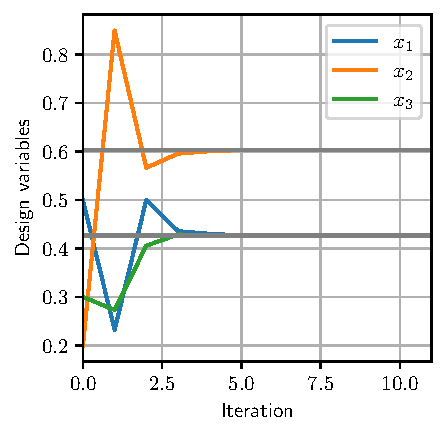
\includegraphics[width=0.9\linewidth]{figures/three_bar_truss_variables.pdf}
    \end{minipage}%
    \begin{minipage}{.5\textwidth}
        \centering
        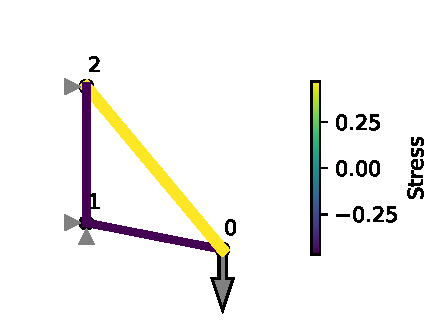
\includegraphics[width=0.9\linewidth]{figures/three_bar_truss_optimized.pdf}
    \end{minipage}
       
\end{example}

\begin{example}{Truss optimization}{trussoptimizationexample}
    The following figure plots the deformed configuration of a sizing optimization result for the truss shown in Figure \ref{fig:truss_example}. Line thicknesses correspond to the design variables and colors indicate stresses. Note that this is not a fully stressed design (the stress magnitudes are not all identical), because some design variables reach their upper limit. Essentially, the outcome is close to a topology optimization, because it indicates elimination of some elements. However, a complete elimination is not possible as this would result in a singular stiffness matrix, i.e. the displacement of node 9 would be undetermined. 

    \begin{center}
        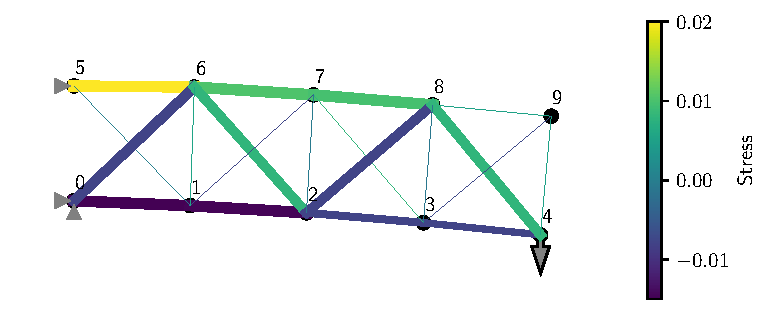
\includegraphics[width=0.9\textwidth]{figures/truss_sample_optimized.pdf} 
    \end{center}
\end{example}

\begin{example}{Large truss optimization}{largetrussoptimizationexample} 
    We could solve very simple truss optimization problems, like the three bar problem above, analytically. Hence, the applied method with MMA seems a bit overkill. 
    However, we cannot solve the optimization problem for large structures like the truss below analytically. 

    \begin{center}
        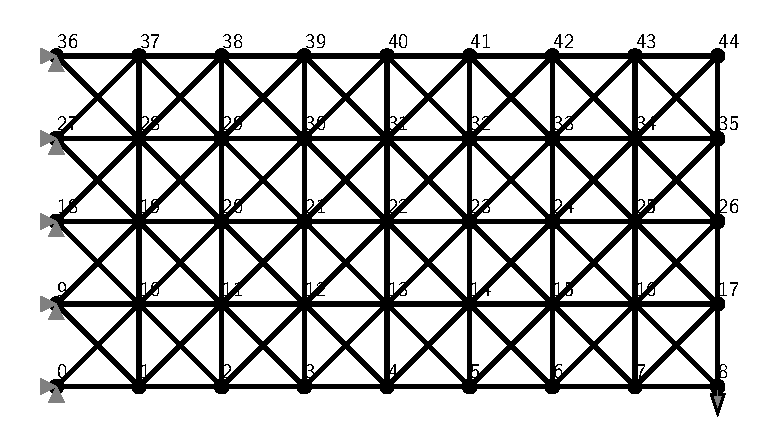
\includegraphics[width=0.75\textwidth]{figures/large_truss.pdf} 
    \end{center}

    In this case, the truss was optimized with large enough upper limits for the cross sections such that the resulting optimized structure is fully stressed. We may interpret the resulting structure effectively as a four bar truss with optimal cross sections. Note that we did not consider instability problems like buckling, so before building a truss structure like this we should check it for buckling instabilities.

    \begin{center}
        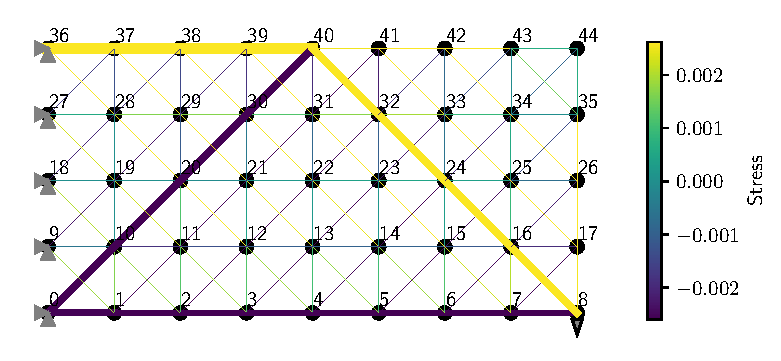
\includegraphics[width=0.9\textwidth]{figures/large_truss_optimized.pdf} 
    \end{center}
\end{example}


\bibliographystyle{unsrtnat}
\bibliography{literature} 